\chapter{Hábitos saludables}\label{ch:g1:healthy-habits}

¿Por qué todo el mundo repite ``lávate las manos'', ``lávate los
dientes'', ``a la cama''? No para estropear la diversión. Tu cuerpo es
el \omterm{def:g1:living-or-not:living}{ser vivo} que conservarás más tiempo --- toda la vida --- y unos
cuantos hábitos pequeños, hechos cada día, lo mantienen fuerte. Estos
son, y esta es la razón de que funcionen.

\section{Estar limpio}

\begin{definition}[Microbios]\label{def:g1:healthy-habits:germs}
Los \emph{microbios}\index{microbio} son \omterm{def:g1:living-or-not:living}{seres vivos} demasiado
pequeños para verlos, que están por todas partes --- en las manos, en
los picaportes, en la tierra. Casi todos son inofensivos, pero algunos
nos pueden poner enfermos si entran en el cuerpo. Como son invisibles,
unas manos que parecen limpias los pueden llevar igualmente.
\end{definition}

\begin{definition}[Higiene]\label{def:g1:healthy-habits:hygiene}
La \emph{higiene}\index{higiene} son los hábitos que mantienen el
cuerpo limpio y dejan fuera a los \omterm{def:g1:healthy-habits:germs}{microbios}: lavarse las manos, lavarse
el cuerpo, lavarse los dientes, cuidar la limpieza de la comida.
\end{definition}

\begin{method}[Lavarse bien las manos]\label{met:g1:healthy-habits:hands}
\begin{enumerate}
  \item mójate las manos y coge jabón;
  \item frota por todas partes --- palmas, dorsos, entre los dedos,
        alrededor de los pulgares --- mientras cuentas despacio hasta
        $20$ o cantas una canción corta;
  \item aclárate con agua corriente;
  \item sécate con una toalla limpia.
\end{enumerate}
Lávatelas antes de comer, después del váter y después de jugar en la
calle o de tocar \omterm{def:g1:animals-around-us:animal}{animales}.
\end{method}

\begin{omfigure}
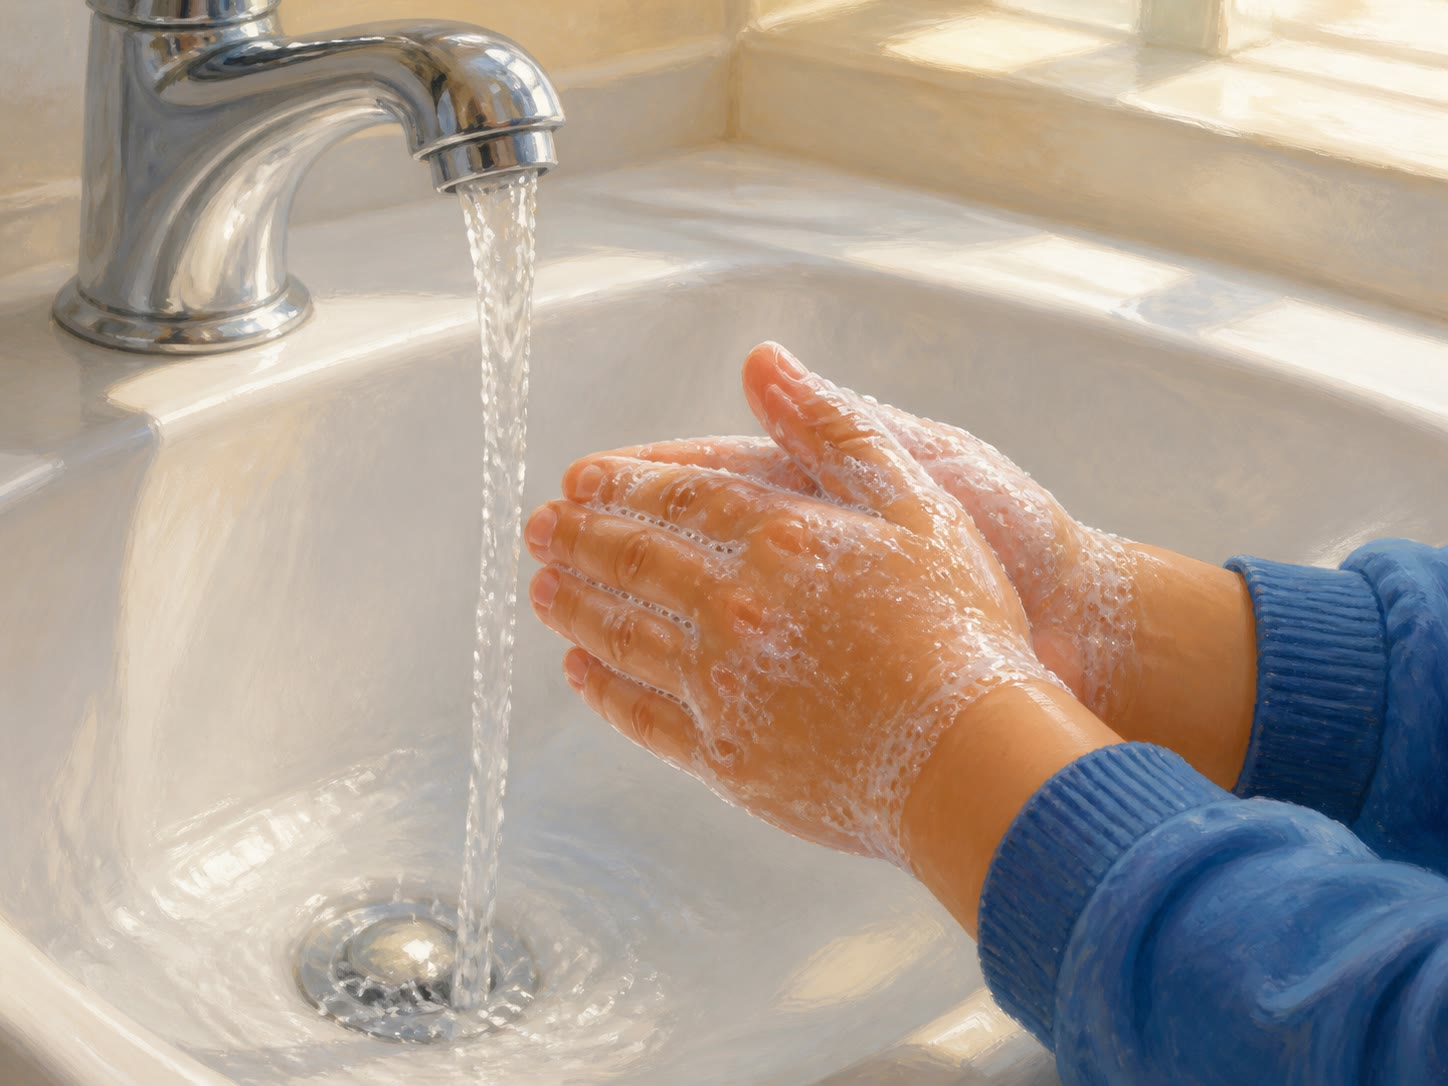
\includegraphics[width=0.58\linewidth]{images/book1/ai/g1-habits-handwashing.jpg}

{\small Jabón, frotar y agua corriente: la canción que menos les gusta
a los \omterm{def:g1:healthy-habits:germs}{microbios} dura veinte cuentas despacio.}
\end{omfigure}

\begin{example}[El experimento de la purpurina]\label{ex:g1:healthy-habits:glitter}
Frótate una pizca de purpurina en las palmas y después dale la mano a
un amigo, abre una puerta, coge un lápiz: purpurina por todas partes.
Los \omterm{def:g1:healthy-habits:germs}{microbios} viajan exactamente así, solo que sin verse. Ahora lávate
con jabón contando hasta $20$ --- se va la purpurina y se van también
los \omterm{def:g1:healthy-habits:germs}{microbios}.
\end{example}

\section{Dientes para toda la vida}

\begin{proposition}[Por qué hay que lavarse los dientes]\label{prop:g1:healthy-habits:teeth}
Después de comer quedan restos de comida en los dientes. Los \omterm{def:g1:healthy-habits:germs}{microbios}
de la boca se alimentan de esos restos --- sobre todo de los dulces
--- y poco a poco hacen agujeros en los dientes, que duelen. El cepillo
barre los restos antes de que los \omterm{def:g1:healthy-habits:germs}{microbios} se den el banquete.
\end{proposition}
\admitted

\begin{method}[Lavarme los dientes]\label{met:g1:healthy-habits:brush}
\begin{enumerate}
  \item lávatelos después del desayuno y antes de acostarte --- cada día;
  \item cepilla todas las caras de todos los dientes: la de delante, la
        de detrás y la de arriba, donde masticas;
  \item tómate tu tiempo --- más o menos lo que dura una canción;
  \item cambia de cepillo cuando las cerdas se abran.
\end{enumerate}
\end{method}

\begin{remark}[Los dientes de leche también cuentan]\label{rem:g1:healthy-habits:babyteeth}
``Estos dientes se van a caer igual --- ¿para qué lavarlos?'' Porque
todavía tienen que masticar por ti durante años, porque los agujeros
duelen exactamente igual y porque los dientes de mayor ya están
esperando debajo y merecen llegar a una boca limpia y sana.
\end{remark}

\section{Comer, moverse, dormir}

\begin{proposition}[Las tres necesidades de cada día]\label{prop:g1:healthy-habits:needs}
Un cuerpo que crece necesita, todos los días:
\begin{enumerate}
  \item \emph{comida variada}\index{comida variada} --- un poco de
        todo: verdura y fruta, pan y cereales, leche y queso, carne o
        pescado o huevos, y agua para beber; dulces solo de vez en
        cuando;
  \item \emph{movimiento}\index{movimiento} --- correr, trepar, montar
        en bici, jugar en la calle: moverse hace más fuertes los
        músculos, los huesos y el corazón;
  \item \emph{sueño}\index{sueño} --- por la noche el cuerpo descansa,
        se repara y crece; un niño necesita una noche larga, mucho más
        larga que la de una persona mayor.
\end{enumerate}
\end{proposition}
\admitted

\begin{omfigure}
\begin{tikzpicture}
  \draw[thick, omMeth, fill=omMeth!7, rounded corners=6pt]
    (0,0) rectangle (3.6,2.3);
  \draw[thick, omProp, fill=omProp!7, rounded corners=6pt]
    (4.0,0) rectangle (7.6,2.3);
  \draw[thick, omDef, fill=omDef!7, rounded corners=6pt]
    (8.0,0) rectangle (11.6,2.3);
  \node[font=\small\bfseries, omMeth] at (1.8,1.95) {comer variado};
  \node[font=\small\bfseries, omProp] at (5.8,1.95) {moverse};
  \node[font=\small\bfseries, omDef] at (9.8,1.95) {dormir};
  \node[font=\small, align=center, text width=3.3cm] at (1.8,0.9)
    {un poco de\\ todo,\\ agua para beber};
  \node[font=\small, align=center, text width=3.3cm] at (5.8,0.9)
    {jugar fuera,\\ correr, trepar,\\ todos los días};
  \node[font=\small, align=center, text width=3.3cm] at (9.8,0.9)
    {una noche larga:\\ el cuerpo se repara\\ y crece};
\end{tikzpicture}

{\small Las tres necesidades diarias de un cuerpo que crece. Ninguna
de las tres puede sustituir a otra.}
\end{omfigure}

\begin{example}[Un buen día para el cuerpo]\label{ex:g1:healthy-habits:day}
Desayuno con fruta; manos lavadas antes de comer; una tarde corriendo
en el parque; dientes lavados después de cenar; luz apagada pronto con
un cuento. Nada extraordinario --- y de eso se trata: la salud está
hecha de días corrientes como este.
\end{example}

\begin{remark}[El cansancio es un mensaje]\label{rem:g1:healthy-habits:tired}
Bostezos, \omterm{def:g1:the-five-senses:sense}{ojos} que escuecen, mal humor sin motivo: eso es el cuerpo
diciendo ``necesito dormir''. Hacerle caso también es un hábito
saludable. Un cerebro que ha dormido bien aprende mejor por la mañana,
juega mejor y se ríe más fácilmente.
\end{remark}

\section{Ejercicios}

\begin{exercise}[$\star$]\label{exo:g1:healthy-habits:1}
¿Qué son los \omterm{def:g1:healthy-habits:germs}{microbios}? ¿Por qué unas manos que parecen limpias pueden
necesitar lavarse igualmente?
\end{exercise}

\begin{exercise}[$\star$]\label{exo:g1:healthy-habits:2}
Di tres momentos del día en los que hay que lavarse las manos.
\end{exercise}

\begin{exercise}[$\star$]\label{exo:g1:healthy-habits:3}
En el \cref{met:g1:healthy-habits:hands}, ¿cuánto tiene que durar el
frotado con jabón? Nombra dos sitios que se olvidan fácilmente.
\end{exercise}

\begin{exercise}[$\star$]\label{exo:g1:healthy-habits:4}
¿Por qué se hacen agujeros en los dientes cuando no se lavan? Cuenta
la historia con los \omterm{def:g1:healthy-habits:germs}{microbios} y los restos de comida.
\end{exercise}

\begin{exercise}[$\star$]\label{exo:g1:healthy-habits:5}
¿Cuándo hay que lavarse los dientes y cuánto tiene que durar?
\end{exercise}

\begin{exercise}[$\star$]\label{exo:g1:healthy-habits:6}
Nombra las tres necesidades diarias de la
\cref{prop:g1:healthy-habits:needs} y un ejemplo de cada una de tu
propio día.
\end{exercise}

\begin{exercise}[$\star$]\label{exo:g1:healthy-habits:7}
¿Qué hace el cuerpo mientras duermes? ¿Quién necesita la noche más
larga, un niño o una persona mayor?
\end{exercise}

\begin{exercise}[$\star$]\label{exo:g1:healthy-habits:8}
Da dos señales de que un cuerpo está pidiendo dormir.
\end{exercise}

\begin{exercise}[$\star\star$]\label{exo:g1:healthy-habits:9}
Sam dice: ``Mis dientes de leche se van a caer igual, así que lavarlos
no sirve de nada''. Respóndele con la
\cref{rem:g1:healthy-habits:babyteeth} --- al menos dos razones.
\end{exercise}

\begin{exercise}[$\star\star$]\label{exo:g1:healthy-habits:10}
En el experimento de la purpurina del
\cref{ex:g1:healthy-habits:glitter}, ¿qué representa la purpurina?
¿Qué demuestra el experimento sobre darse la mano --- y sobre el jabón?
\end{exercise}
